% !TEX root =../thesis-letomes.tex

\chapter{Literature Overview}
\section{LETOs – A Historic Overview}
The concept of low energy transfer orbits can be traced back to conference proceedings in in 1987, where Edward Belbruno first suggested it as a cheaper way to the moon under the constraint of using just electric propulsion (a class of engines known for their high efficiency but low thrust). It turned out to be possible, at least in theory, although the trip would take nearly 2 years. \cite{Belbruno1987} \cite{Benson}.

The concept of LETOs was first tried in 1990 to manuever the Japanese spacecraft Hiten to the Moon. Japan had launched two spacecraft into Earth's orbit, Hiten and Hagoromo. Hiten was just meant as a relay satellite and Hagoromo was supposed to go to the Moon via a standard Hohmann transfer (takes about 4 days), but never made it. The Hiten only had 10\% of the fuel needed for a Hohmann transfer. The Japanese team was desperate to try anything to make something interesting out of their mission, so they contacted Belbruno, who designed an orbit with colleague James K. Miller from JPL that could get Hiten to the Moon in 4 months down from 2 years by taking the Sun's constant force into consideration. The maneuver was a success \cite{Belbuno1990} \cite{Benson}. \cref{fig:hiten} shows the trajectory.

\begin{figure}[ht]
    \centering
    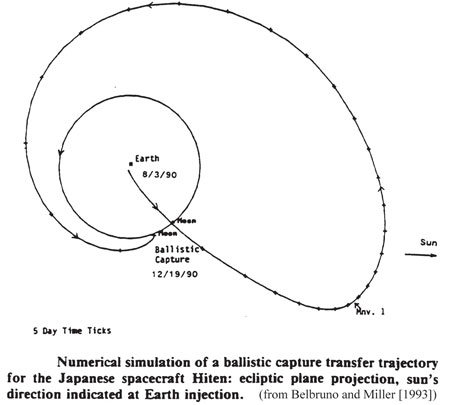
\includegraphics[width=0.50\linewidth]{fig/hiten.png}
    \caption{The Hiten spacecraft performed the first attempt at a LETO to the Moon ever in 1990, and was a success.}
    \label{fig:hiten}
\end{figure}

After Hiten, a small number of missions have utilized LETOs in their missions:
\begin{itemize}
	\item SMART-1 (ESA, 2003--2006): Was used to test solar electric propulsion and other deep-space technologies, while performing scientific observations of the Moon before deliberately crashing into it \cite{ESA}. Used electric propulsion to gradually make it's way to the moon along a LETO.
    \item Genesis (NASA, 2001--2004): Collect solar wind samples at the Earth-Sun L1 Lagrange point and returned them to Earth for study \cite{NASAa}.
\end{itemize}
